\section{Ancho de banda de memoria y capacidad de cómputo para el kernel \texttt{saxpy}}

Queremos obtener el rendimiento del ancho de banda de memoria y la capacidad de cómputo para nuestra
GPU con el código \texttt{saxpy}.

\begin{table}[H]
	\centering
	\begin{tabular}{|l|l|}
	\hline
	CPU               & AMD Ryzen 7 2700X                 \\ \hline
	RAM               & 32GB 2133MHz CL15				  \\ \hline
	GPU               & NVIDIA GeForce RTX 2060           \\ \hline
	Controlador GPU   & 31.0.15.3168                      \\ \hline
	Sistema Operativo & Windows 10 Pro 21H2 19044.2965    \\ \hline
	Compilador        & Visual Studio 2022 versión 17.5.5 \\ \hline
	\end{tabular}
	\caption{Especificaciones del ordenador en que se ejecutan los experimentos.}
\end{table}

\begin{figure}[H]
    \centering
    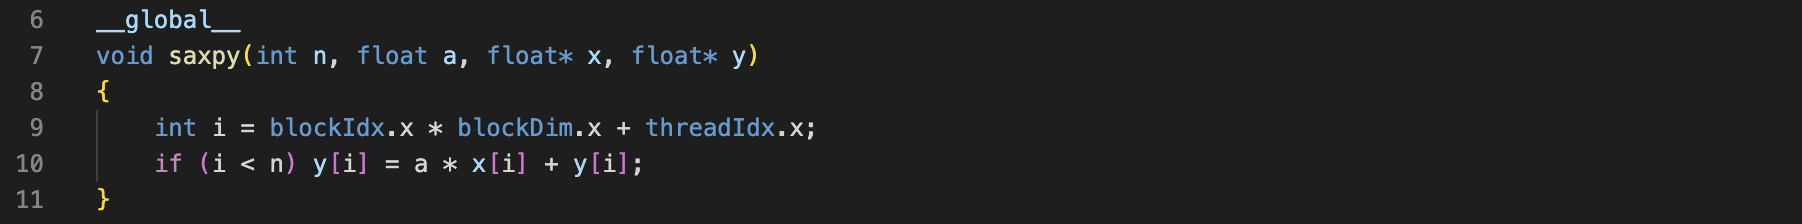
\includegraphics[width=\textwidth]{saxpy.png}
    \caption{Código de ejemplo \texttt{saxpy} que encontramos en \url{https://developer.nvidia.com/blog/how-implement-performance-metrics-cuda-cc/}
	Extraemos los recursos que utilizamos de esta página web.}
\end{figure}

\subsection{Ancho de banda de memoria.}

Para calcular el ancho de banda de memoria teórico utilizamos la fórmula

$$ BW_{Theorical} = T \cdot R $$

siendo $T$ el número de transferencias efectuadas por unidad de tiempo y $R$ la relación $\frac{bytes}{transferencia}$.

Por otra parte, para el cálculo del ancho de banda efectivo, tenemos que

$$ BW_{Effective} = \frac{R_{B} + W_{B}}{t} $$

donde $R_{B}$ es el número de bytes leídos por kernel y $W_{B}$ es el número de bytes
escritos por kernel.

\pagebreak

Nuestra gráfica utiliza memoria una memoria GDDR6, es decir, memoria de tipo \textit{double data rate},
y con una interfaz de memoria de 192 bits, funcionando a $1.75GHz$ en frecuencia base y $14GHz$ en la efectiva.

Para una \textit{RTX 2060} tenemos que

$$ BW_{Theorical} = 336 \ \frac{GB}{s} $$

si tomamos como la velocidad de la memoria la efectiva.

Por otra parte, tras ejecutar el programa, para la misma gráfica obtenemos un ancho de banda

$$ BW_{Effective} = 148.271504 \ \frac{GB}{s} $$

\subsection{Capacidad de cómputo.}

Desconocemos el máximo teórico de operaciones en coma flotante por unidad de tiempo para la \textit{RTX 2060}, pero calculamos el efectivo de la siguiente forma.

$$ GFLOPS = \frac{2 \cdot N}{t \cdot 10^{9}} = 2.471192 \ GFLOPS $$

Donde $N$ es el número de operaciones en coma flotante y $t$ el tiempo transcurrido en segundos.

